\documentclass[10pt,aspectratio=43]{beamer}

\usepackage{graphicx}
\usepackage{tikz}
\usepackage{xcolor}
\usepackage{caption}
\usepackage{subcaption}
\usepackage{bm}
\usetikzlibrary{calc} 
\usepackage{hyperref}
\hypersetup{
    colorlinks=true,
    linkcolor=blue,
    urlcolor=red
}
\usepackage{fontawesome5}
\usepackage{ulem}

\usetheme{MyStyle}   % loads beamerthemeMyStyle.sty
\setlength{\columnsep}{0pt}


%%%%%%%%%%%%%%%%%%%%%%%%%%%%%%%%%%%%%%%%%%
%%%%%%%%%%%%%%%%%%%%%%%%%%%%%%%%%%%%%%%%%%
%%%%%%%%%%%%%%%%%%%%%%%%%%%%%%%%%%%%%%%%%%

\title{Pull request status}
\newcommand{\eventname}{ALERT meeting}
\author{Felix Touchte Codjo}
\institute{IJCLab}
\date{\today}


\begin{document}

\begin{frame}[plain] % remove header, footer, barre de navigation
\titlepage
\end{frame}

%\begin{frame}{Outline}
%\tableofcontents
%\end{frame}

%\section{Intro}
\section{Updates}

\begin{frame}{Pull request status}
    \begin{itemize}
        \item Incoming pull requests
            \begin{enumerate}
                \item Add routine to clean bad AHDC hits and Use ATOF hits in the Kalman Filter
                    \begin{itemize}
                        \item[$\circ$] It is more difficult than expected
                        \item[$\circ$] A lot of divergences of {\color{red} \texttt{coatjava/development}}, especially with ALERTEngine and Track
                    \end{itemize}
            \end{enumerate}
    \end{itemize}

    \centering
    \vspace{0.2cm}

    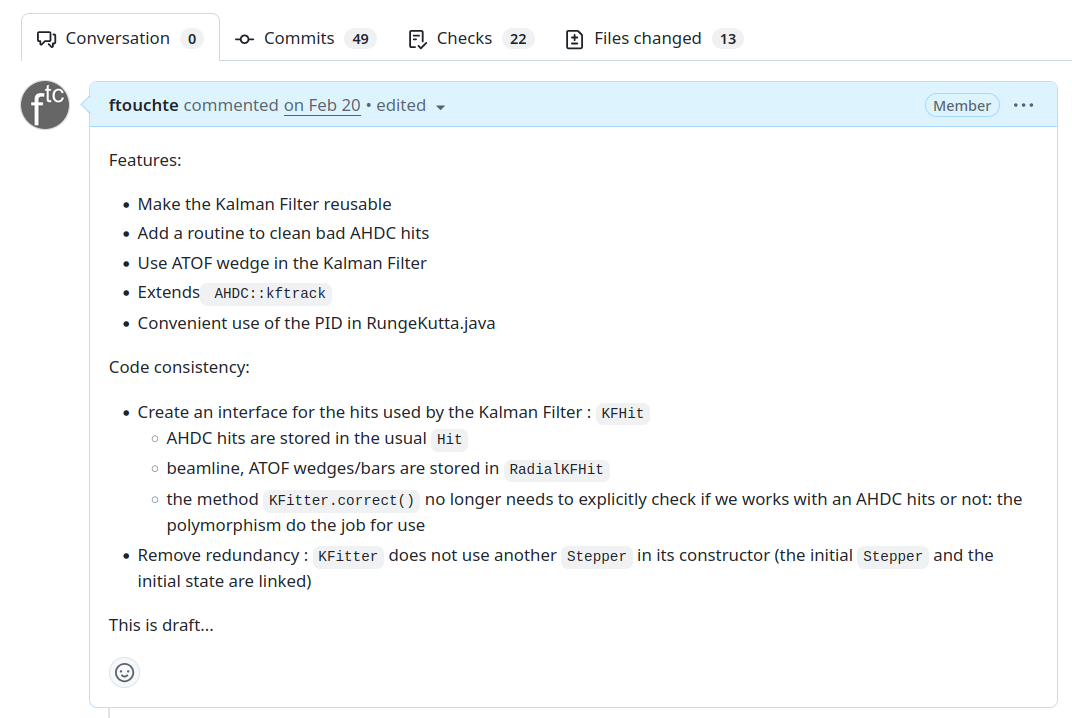
\includegraphics[width=0.7\linewidth]{figures/pending-pr.png}
\end{frame}

\begin{frame}[fragile]{Pull request status}
    \begin{itemize}
        \item Incoming pull requests
            \begin{enumerate}
                \item[2.] Layer and wire alignment implementation
                    \begin{itemize}
                        \item[$\circ$] It is easier, but I need to validate the structure of the tables
                         \item[$\circ$] For the wire alignment, the angles are relative to the layers
                    \end{itemize}
            \end{enumerate}
    \end{itemize}

    \centering
    \vspace{0.5cm}

    \begin{minipage}{0.45\textwidth} \tiny
        \begin{verbatim}
# geometry/alert/ahdc/layer_alignment
# sector, layer, angle_start, angle_end
 1   11   0.875600   0.814700
 1   21   0.965500   0.760600
 1   22   0.553000   0.373300
 1   31   0.738500   0.768000
 1   32   0.392600   0.443200
 1   41   0.479700   0.481400
 1   42   0.252700   0.327400
 1   51   0.467300   0.219300
        \end{verbatim}
    \end{minipage}
    \begin{minipage}{0.45\textwidth} \tiny
        \begin{verbatim}
# geometry/alert/ahdc/wire_alignment
# sector, layer, wire, angle
 1   11    1   0.000000
 1   11    2   0.000000
 1   11    3   0.000000
 1   11    4   0.000000
 1   11    5   0.000000
 1   11    6   0.000000
 1   11    7   0.000000
 1   11    8   0.000000
 1   11    9   0.000000
 1   11   10   0.000000
 1   11   11   0.000000
 1   11   12   0.000000
 1   11   13   0.000000
 ...
 1   51   95   0.000000
 1   51   96   0.000000
 1   51   97   0.000000
 1   51   98   0.000000
 1   51   99   0.000000
        \end{verbatim}
    \end{minipage}

    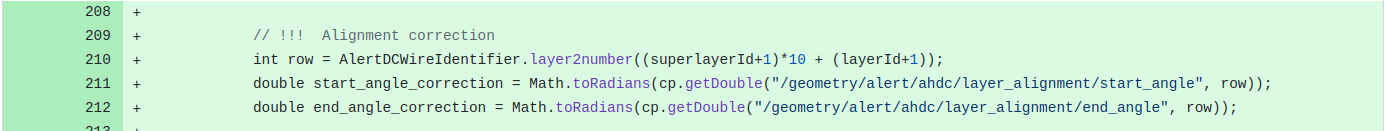
\includegraphics[width=0.7\linewidth]{figures/use-constant-provider.png}

\end{frame}





\end{document}


